\documentclass[%
 reprint,
%superscriptaddress,
%groupedaddress,
%unsortedaddress,
%runinaddress,
%frontmatterverbose, 
%preprint,
%preprintnumbers,
%nofootinbib,
%nobibnotes,
%bibnotes,
 amsmath,amssymb,
 aps,
%pra,
%prb,
%rmp,
%prstab,
%prstper,
%floatfix,
]{revtex4-2}

\usepackage{graphicx}% Include figure files
\usepackage{dcolumn}% Align table columns on decimal point
\usepackage{bm}% bold math
\usepackage{float}
\usepackage{caption}
%\usepackage{hyperref}% add hypertext capabilities
%\usepackage[mathlines]{lineno}% Enable numbering of text and display math
%\linenumbers\relax % Commence numbering lines

%\usepackage[showframe,%Uncomment any one of the following lines to test 
%%scale=0.7, marginratio={1:1, 2:3}, ignoreall,% default settings
%%text={7in,10in},centering,
%%margin=1.5in,
%%total={6.5in,8.75in}, top=1.2in, left=0.9in, includefoot,
%%height=10in,a5paper,hmargin={3cm,0.8in},
%]{geometry}
\let\olditemize\itemize
\def\itemize{\olditemize\itemsep=0pt }

\begin{document}


\preprint{APS/123-QED}

\title{Una acercamiento hacia el Big Bang}% Force line breaks with \\



 \author{Carlos Andrés Betancur}
 \altaffiliation[Also at ]{Instituto de física, Universidad de Antioquia.}


\affiliation{%
 Instituto de física, Universidad de Antioquia
}%


\date{Diciembre 10, 2020}% It is always \today, today,
             %  but any date may be explicitly specified
\begin{abstract}

\end{abstract}


\maketitle

%\tableofcontents

\section{\label{sec:level1}Resumen}
Las partículas elementales en la naturaleza pueden obtenerse por medio de la colisión entre protones que se mueven con una alta energía, mediante esta técnica pueden ser obtenidos quarks, leptones, bosones, etc. El conocer las partículas elementales constituyentes de la materia nos puede brindar una idea acerca del origen de nuestro universo y lo sucedido en los primeros instantes luego de la explosión del Big Bang.\\
\\
\textbf{Palabras Clave}: Positrón, hadrón, colisionador, quark, LHC.

\section{\label{sec:level1}Introducción }
\\
Por milenios el hombre se ha preguntado sobre el pasado de nuestro universo ¿Cómo ha surgido? ¿Cómo evoluciona? ¿Cuál será su destino? estas han sido preguntas inquietantes que gracias a los curiosos de la ciencia han podido ser respondidas con sólidos argumentos basados en experimentación científica. En este texto particularmente trataremos la primera pregunta, el origen de nuestro universo y las primeras partículas que habitaron en él. Para entender esto debemos comprender los constituyentes de la materia, no fue sino hasta el siglo V a.c que la escuela atomista de la Antigua Grecia postula que la materia está compuesta de átomos y establece que éste es un bloque básico e indivisible siendo Demócrito uno de sus más grandes exponentes[1], siglos más tarde este concepto del átomo como un objeto indivisible tuvo que ser reconsiderado gracias al ingeio del científico J.J Thomson (1856-1940) quien el 30 de abril de 1897 anuncia el descubrimiento de un corpúsculo al que llamó electrón (partícula caracterizada por tener carga negativa) y probó que este era un constituyente para todos los átomos[2]. Años más tarde hacia  1918, el químico y físico británico Ernest Rutherford (1871-1937) descubre la existencia de una nueva partícula subatómica a la que llamó protón (caracterizada por tener carga positiva)[3]. fue a partir de este momento que se empezaron a construir modelos para el átomo que estaría conformado por estas pequeñas partículas. \\
\\
\begin{figure}[H]
\begin{center}
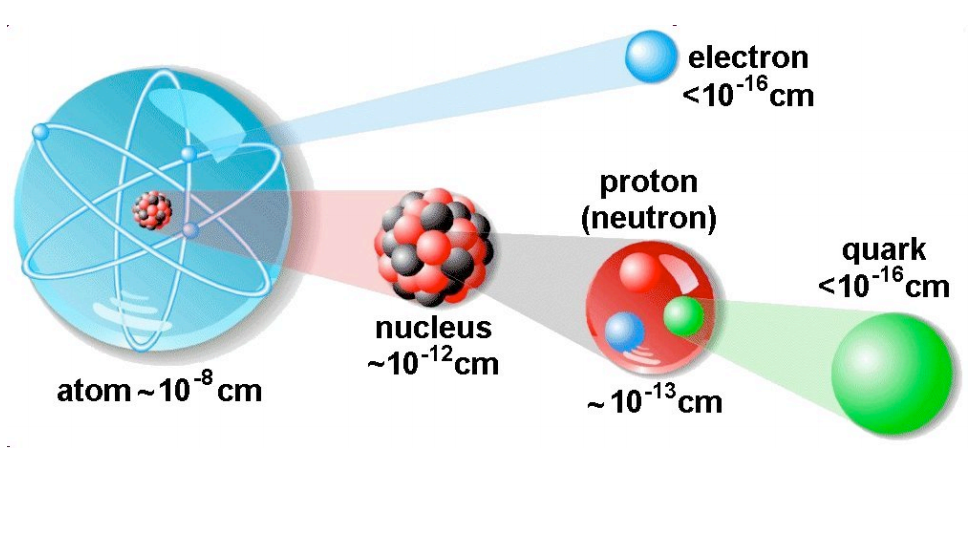
\includegraphics[scale=0.2]{Constituyentes de la materia.png}
\caption{Constituyentes de la materia}\\
\centering
\end{center}
\end{figure}

\\
 sin embargo todo no acaba aquí, con las investigaciones en física de altas energías se descubre que el protón está conformado a su vez partículas más pequeñas llamadas hadrones que resultan de la interacción nuclear fuerte entre los quarks, las cuales han sido consideradas al día de hoy como las verdaderas partículas elementales ya que se desconoce su estructura interior.\\
\section{\label{sec:level1}Obteniendo las partículas elementales}
En 1964, dos físicos Murray Gell Mann y George Zweig propusieron cada uno por su lado la existencia de nuevas partículas subatómicas conocidas como quarks, años más tarde se pudo probar la existencia de estas partículas mediante la colisión de positrones que se aniquilan emitiendo un fotón y produciendo luego un quark y un antiquark.\\
\\
\begin{figure}[H]
\begin{center}
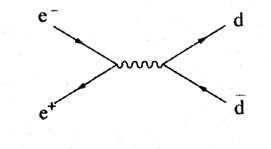
\includegraphics[scale=0.86]{figure1_8.jpeg}
\caption{Colision de hadrones}\\
\centering
\end{center}
\end{figure}
\\
Para conseguir esto se ponen átomos de hidrógeno en la fuente de un gran acelerador en donde se les arrancan los electrones que orbitan a estos átomos quedando así unicamente positrones de hidrógeno en dicha fuente, posteriormente se aceleran estos protones (núcleos de hidrógeno) haciendo uso de un campo eléctrico, luego se introducen en un tubo con forma circular y se aceleran nuevamente mediante un campo eléctrico pulsante (técnica resonante)[5] y el uso de imanes extremadamente potentes que hacen una fuerza perpendicular al movimiento de los positrones, el campo electrico pulsante acelera los protones hasta el $ 91,6\%$ de la velocidad de la luz haciendo cada vez más compacto el paquete de protones que luego se redirige hacia un ciclotron donde revolucionan hasta alcanzar una velocidad cercana a la velocidad de la luz, se alcanza el punto de transicion, es decir los protones están preparados para introducirse en un super ciclotrón donde conseguirán una velocidad cercana a la velocidad de la luz, se harán por tanto más pesados y tendrán la energía suficiente para ser dirigidos al gran colisionador de hadrones (LHC) donde se hacen circular unos en direccion de las manecillas del reloj y otros en sentido contrario de modo que al colisionar se libera una gran energía que producirá estados similares a los que se dieron luego del Big Bang y emergen entonces estas partículas elementales

\begin{figure}[H]
\begin{center}
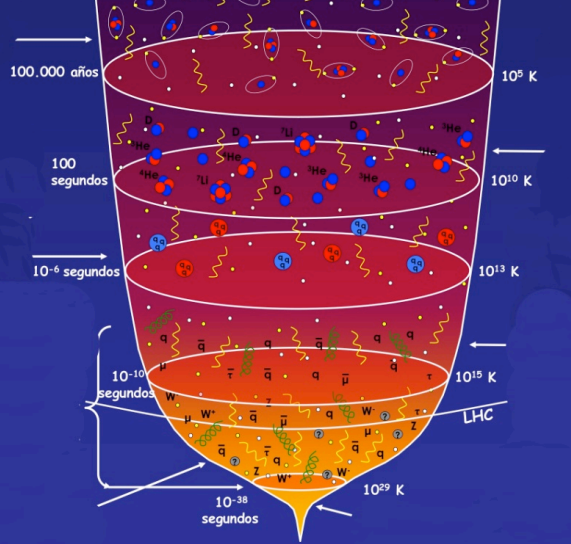
\includegraphics[scale=0.4]{bb.png}
\caption{Primeros instantes del universo}\\
\centering
\end{center}
\end{figure}
\\
 
\section{\label{sec:level1}Resultados}

Al acelerar los hadrones e inyectarles cierta cantidad de energía y hacerlos colisionar esto hará que se rompa su estructura interna liberando así fotones que posteriormente decaen en una partícula que tenga disponible la suma de la energía de ambos rayos. para analizar estas colisiones se ponen unos detectores en el punto de colisión. En el caso del LHC se tienen detectores como el ATLAS el cual es uno de los dos detectores de uso general, Estudia el bosón de Higgs y busca signos de nueva física de partículas, incluidos los orígenes de la masa y las posibles dimensiones adicionales, el CMS (detector de uso general, como ATLAS) estudia el bosón de Higgs y busca pistas para nuevos descubrimientos físicos y nuevas partículas; ALICE está estudiando una forma de materia muy "fluida" llamada plasma quark-gluón que se cree existió poco después del Big Bang; y el LHCb investiga lo que le sucedió a la antimateria "desaparecida" ya que durante el Big Bang se crearon cantidades iguales de materia y antimateria[4].

\begin{figure}[H]
\begin{center}
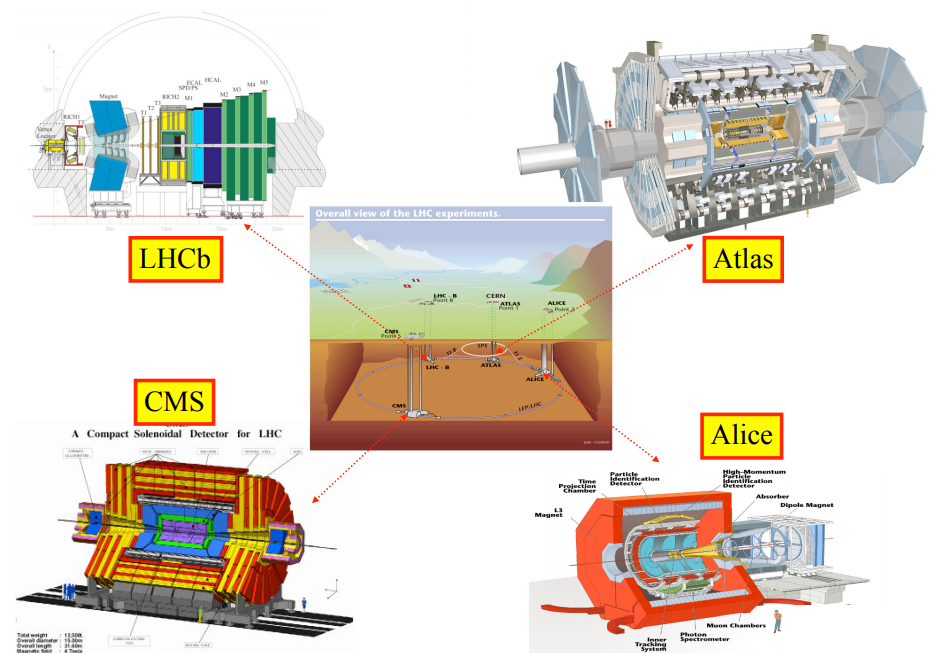
\includegraphics[scale=0.26]{detectores.png}
\caption{Detectores del LHC}\\
\centering
\end{center}
\end{figure}

Estos detectores obtienen unos datos y capturan unas fotos que tienen un comportamiento cualitativo característico dependiendo de la energía del hadrón, como ejemplo podemos tomar la partícula Z la cual es obtenida cuando se logra hacer colisionar los hadrones hasta una energía de 91GeV.

\begin{figure}[H]
\begin{center}
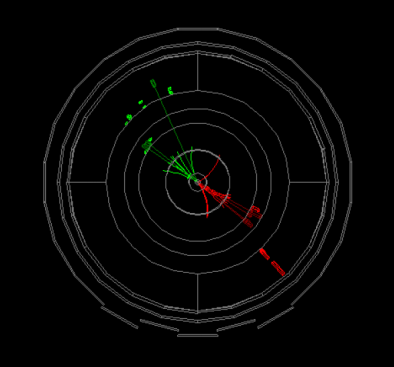
\includegraphics[scale=0.4]{Z.png}
\caption{Desintegración de una partícula Z}\\
\centering
\end{center}
\end{figure}

En la figura 5 el centro geométrico coincide con el punto donde los hadrones colisionan y las trayectorias resultantes serán un indicador de la partícula en la cual está decayendo.

\section{\label{sec:level1}Conclusiones}

En general no es fácil obtener estas partículas ya que esta técnica de colisiones requiere de mucha energía lo que se traduce en un alto costo económico.\\

Al colisionar hadrones a muy altas energías podemos tener un acercamiento a los que sucedía en los primeros instantes del universo (alrededor de $10^-{10} s$) y tener una idea de las partículas elementales que constituyen la materia.

\section{\label{sec:level1} Referencias.}

1. Atomo, tomado de https://es.wikipedia.org/wiki/Átomo, recuperado en diciembre 10 del 2020\\
\\
2. Raymond A. Serway, Clement J. Moses, Curta A. Moyer, Modern Physic-The particle nature of matter, Third edition, Pag 106, Editorial Thomson, printed 2005, United States of America.\\
\\
3. Robert M. Eisberg, Fundamentos de física moderna, El descubrimiento del núcleo atómico, universidad de California, Printed 2000, Editorial Limusa, México\\
\\
4. Gran colisionador de hadrones, tomado de https://es.wikipedia.org/wiki/Gran\_colisionador\_de\_hadrones, recuperado en diciembre 10 del 2020\\
\\
5. Raymond A. Serway, Clement J. Moses, Curta A. Moyer, Modern Physic-Elementary particles, Third edition, Pag 564, Editorial Thomson, printed 2005, United States of America.
\\
\\
\\
\\
\\
\\
\\
\\
\\
\\
\\
\\
\\
\\
\\
\\
\\
\\
\\
\\
\\
\\
\\
\\
\\
\\
\\
\\
\\
\\
\\
\\
\\
\\
\\
\\
\\
\\
\\
\\
\\
\\
\end{document}
